% --------------------------------------------------------------
% This is all preamble stuff that you don't have to worry about.
% Head down to where it says "Start here"
% --------------------------------------------------------------

\documentclass[11pt]{article}
\usepackage[margin=1in]{geometry}
\usepackage{amsmath,amsthm,amssymb}
%\usepackage{multicol}
\usepackage{graphicx}
%\usepackage{fixltx2e}
%\usepackage{amsmath}

\usepackage{tikz}
\usepackage{pgfplots}
\usepackage{heuristica}
\usepackage[heuristica,vvarbb,bigdelims]{newtxmath}
\usepackage[T1]{fontenc}
\usepackage[inline]{enumitem}
\usepackage{subcaption}



%\everymath{\displaystyle}

\newcommand\ft{Fourier transform}
\newcommand\ift{inverse Fourier transform}
\newcommand\ftr{Fourier transform representation}
\newcommand\fs{Fourier series}
\newcommand\fsr{Fourier series representation}
\newcommand\xt{$x(t)$}
\newcommand\xo{$X(j\omega)$}
\newcommand\dtfs{discrete-time Fourier series}

\title{\Large Department of Electronic and Telecommunication Engineering\\University of Moratuwa\\Sri Lanka\\{\LARGE \bf \textsc{EN1060 Signals and Systems: Tutorial 06 Discreet-Time Fourier Transfrom \footnote{All the questions are from Oppenheim \emph{et al.} chapter 4.}}}}

\date{\vspace{-0.2in}\today}


\newcommand{\N}{\mathbb{N}}
\newcommand{\Z}{\mathbb{Z}}

\begin{document}



\maketitle
\noindent \tikz \draw (0,0) -- (\textwidth,0);

\begin{enumerate}
    % Q01 Oppenheim et al. p. 361
    \item Write the synthesis and analysis equation for the discrete-time Fourier transform.

    % Q01 Oppenheim et al. p. 362
    \item Consider the signal
        \begin{equation*}
            x[n] = a_nu[n], |a| <1.
        \end{equation*}
        \begin{enumerate}
            \item Express its DTFT $X\left(e^{j\omega}\right)$.
            \item Sketch the magnitude and phase of $X\left(e^{j\omega}\right)$ when $a>0$.
            \item Sketch the magnitude and phase of $X\left(e^{j\omega}\right)$ when $a<0$.
        \end{enumerate}
    \item Express the DTFT of
        \begin{equation*}
            x[n] = a^{|n|}, |a|<1,
        \end{equation*}
        and sketch.
    \item Express the DTFT of
        \begin{equation*}
            x[n] = \begin{cases}1, & |n| \leq N_1\\0, & |n| > N_1\end{cases}
        \end{equation*}
        and sketch it for $N_1 = 2$.
    \item Express and sketch the DTFT of $x[n] = \cos \omega_0 n$.
    \item Express and sketch the DTFT of the discrete-time periodic impulse train $x[n] = \sum_{k=-\infty}^{+\infty}\delta[n - kN]$.

    % Oppenheim q5.21
    \item Compute the \ft of each of the following signals:
    	\begin{enumerate}
    		\item $x[n] = u[n-2] - u[n-1]$
    		\item $x[n] = \left(\frac{1}{2}\right)^{-n}u[-n-1]$
    		\item $x[n] = \left(\frac{1}{3}\right)^{|n|}u[-n-2]$
    		\item $x[n] = \begin{cases}
    		n, & -3 \leq n \leq 3\\ 0, &\text{otherwise}.
    		\end{cases}$
    	\end{enumerate}
    	
    % Oppenheim q5.22
    \item The following are the Fourier transforms of discrete-time signals. Determine the signal corresponding to each transform.
	    \begin{enumerate}
	    	\item $X\left(e^{j\omega}\right) = \begin{cases}
	    	1, &\frac{\pi}{4} \leq |\omega| \leq \frac{3\pi}{4} \\ 0, & \frac{3\pi}{4} \leq |\omega| \leq \pi, 0 \leq |\omega| < \frac{\pi}{4} \end{cases}$
	    	\item $X\left(e^{j\omega}\right) = 1 + 3e^{-j\omega} + 2e^{-j2\omega} -4e^{-j3\omega} + e^{-j10\omega}$
	    	\item $X\left(e^{j\omega}\right) = e^{-j\omega/2}$ for $-\pi \leq \omega \leq \pi$
	    	\item $X\left(e^{j\omega}\right) = \frac{e^{-j\omega} - \frac{1}{5}}{1-\frac{1}{5}e^{-j\omega}}$	    	
	    \end{enumerate}

    % Oppenheim p. 373
    \item Show that 
        \begin{equation*}
            X\left(e^{j(\omega + 2\pi)}\right) = X\left(e^{j\omega}\right).
        \end{equation*}
        Is the continuous-time Fourier transform always periodic as the DTFT?
    % Oppenheim p. 379
    \item Fig. \ref{fi:example59} shows a sequence $x[n]$ adn $y[n]$. 
    \begin{enumerate}
    	\item Express $x[n]$ using subsampled versions of $y[n]$.
    	\item Express $Y\left(e^{j\omega}\right)$.
    	\item Hence, express $X\left(e^{j\omega}\right)$.    	
    \end{enumerate}
    



 	\begin{figure}
		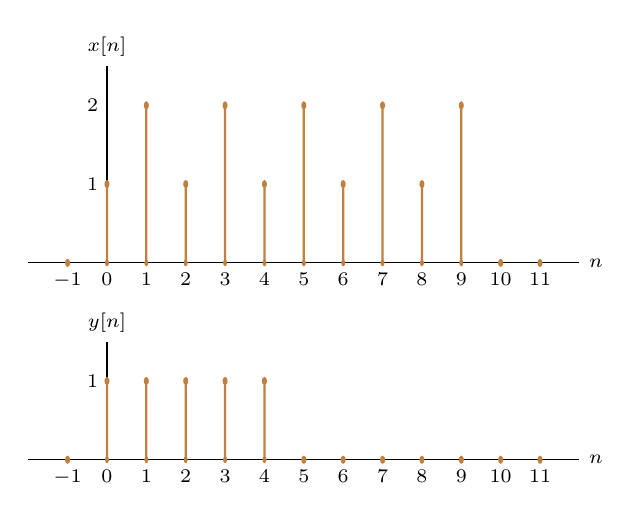
\begin{tikzpicture}[xscale=0.5]




	\def\nmin{-1}
	\def\nmax{11}	
	
	\begin{scope}	
		\def\x{{0, 1, 2, 1, 2, 1, 2, 1, 2, 1, 2, 0, 0}}	

		\draw (\nmin-1, 0) -- (\nmax+1, 0) node[anchor=west] {\scriptsize $n$};
		\draw (0,0) -- ++(0, 2.5) node [anchor=south] {\scriptsize $x[n]$};
% 		\foreach \n/\l in {-1/{-N_1}, 1/0, 3/{N_1}}
% 		{
% 			\node at (\n/4, 0) [anchor=north] {\scriptsize $\l$};
% 		}
		\foreach \n in {-1, 0, ..., 11}
		{
			\node at (\n, 0) [anchor=north] {\scriptsize $\n$};
		}
		\node at (-0.75,1) [anchor=west] {\scriptsize $1$};
		\node at (-0.75,2) [anchor=west] {\scriptsize $2$};
		
		\foreach \n in {0,1, ..., 12}
		{
			\pgfmathparse{\x[\n]}
			\edef\xn{\pgfmathresult}	
			\ifthenelse{\xn > 0}
			{
				\draw[brown, thick, fill=brown]  (\n + \nmin, 0) -- ++(0, \xn) circle (1pt);% node[anchor=east] {\scriptsize $\xn$};
			}
			{
				\draw[brown, fill=brown] (\n+ \nmin,  0) circle (1pt);
			}
		}
	\end{scope}		
	
	\begin{scope}[yshift=-2.5cm]	
		\def\x{{0, 1, 1, 1, 1, 1, 0, 0, 0, 0, 0, 0, 0}}	

		\draw (\nmin-1, 0) -- (\nmax+1, 0) node[anchor=west] {\scriptsize $n$};
		\draw (0,0) -- ++(0, 1.5) node [anchor=south] {\scriptsize $y[n]$};
% 		\foreach \n/\l in {-1/{-N_1}, 1/0, 3/{N_1}}
% 		{
% 			\node at (\n/4, 0) [anchor=north] {\scriptsize $\l$};
% 		}
		\foreach \n in {-1, 0, ..., 11}
		{
			\node at (\n, 0) [anchor=north] {\scriptsize $\n$};
		}
		\node at (-0.75,1) [anchor=west] {\scriptsize $1$};

		
		\foreach \n in {0,1, ..., 12}
		{
			\pgfmathparse{\x[\n]}
			\edef\xn{\pgfmathresult}	
			\ifthenelse{\xn > 0}
			{
				\draw[brown, thick, fill=brown]  (\n + \nmin, 0) -- ++(0, \xn) circle (1pt);% node[anchor=east] {\scriptsize $\xn$};
			}
			{
				\draw[brown, fill=brown] (\n+ \nmin,  0) circle (1pt);
			}
		}
	\end{scope}	
\end{tikzpicture}
		\caption{Sequences}
		\label{fi:example59}
	\end{figure}

	\item Let $X\left(e^{j\omega}\right)$ denote the \ft of the signal shown in Fig. \ref{fi:p523}. Perform the following calculations wihtout explicitly evaluating $X\left(e^{j\omega}\right)$:
 	\begin{figure}
		\begin{tikzpicture}[xscale=0.5]




	\def\nmin{-12}
	\def\nmax{14}	
	
	\begin{scope}	
		\def\x{{0, 0, 0, 0, 0, 0, 0, 0, 0, -1, 0, 1, 2, 1, 0, 1, 2, 1, 0, -1, 0, 0, 0, 0, 0, 0, 0}}	
		\draw (\nmin-1, 0) -- (\nmax+1, 0) node[anchor=west] {\scriptsize $n$};
		\draw (0,0) -- ++(0, 2.5) node [anchor=south] {\scriptsize $x[n]$};
% 		\foreach \n/\l in {-1/{-N_1}, 1/0, 3/{N_1}}
% 		{
% 			\node at (\n/4, 0) [anchor=north] {\scriptsize $\l$};
% 		}
		\foreach \n in {-3, -2, ..., 8}
		{
			\node at (\n, 0) [anchor=north] {\scriptsize $\n$};
		}
		\node at (-0.75,1) [anchor=west] {\scriptsize $1$};
		\node at (-0.75,2) [anchor=west] {\scriptsize $2$};
		
		\foreach \n in {0,1, ..., 26}
		{
			\pgfmathsetmacro\xn{\x[\n]}
			\pgfmathparse{\xn == 0 ? 1 : 0}	
			\ifthenelse{\pgfmathresult>0}
			{
				\draw[brown, fill=brown] (\n+ \nmin,  0) circle (1pt);

			}
			{
				\draw[brown, thick, fill=brown]  (\n + \nmin, 0) -- ++(0, \xn) circle (1pt);% node[anchor=east] {\scriptsize $\xn$};			
				
			}
		}
	\end{scope}		
	
	
\end{tikzpicture}
		\caption{Sequences}
		\label{fi:p523}
	\end{figure}
	\begin{enumerate}
		\item Evaluate $X\left(e^{j0}\right)$
		\item Find $\angle X\left(e^{j\omega}\right)$
		\item Evaluate $\int_{-\pi}^{\pi}X\left(e^{j\omega}\right)d\omega$
		\item Find $X\left(e^{j\pi}\right)$
		\item Determine and sketch the signal whose \ft is $\mathfrak{Re}\{x(\omega)\}$
		\item Evaluate $\int_{-\pi}^{\pi}\left|X\left(e^{j\omega}\right)\right|^2d\omega$
		\item Evaluate $\int_{-\pi}^{\pi}\left|\frac{dX\left(e^{j\omega}\right)}{d\omega}\right|^2d\omega$		
	\end{enumerate}
	

    
\end{enumerate}

\end{document} 